\documentclass[11pt]{sig-alternate}
\usepackage{tabularx}
\usepackage{graphicx}
\usepackage{blindtext}
\usepackage[utf8]{inputenc}
\usepackage[english]{babel}
\usepackage{lastpage}
\usepackage{comment}
\usepackage{dirtytalk}
\usepackage{xcolor}
\usepackage{hanging}
\usepackage{wrapfig}
\usepackage[backend=biber, style=apa]{biblatex}
\addbibresource{notation.bib}
\usepackage{authblk}
\usepackage{caption}
\usepackage{subcaption}
\usepackage{graphicx,subfigure}
\usepackage{authblk}
\usepackage{fancyhdr}
\usepackage{xurl}
\usepackage{hyperref}
\pagestyle{fancy}
\renewcommand{\headrulewidth}{0pt}
\renewcommand{\footrulewidth}{0pt}
\setlength\headheight{80.0pt}
\addtolength{\textheight}{-80.0pt}
\chead{%
  \ifcase\value{page}
  % empty test for page = 0
  \or 
\includegraphics[width=\textwidth]{headerImage.png}% page=1
  \or 
\includegraphics[width=\textwidth]{headerImage.png}% page = 2
  \or 
\includegraphics[width=\textwidth]{headerImage.png}% page = 3
  \or 
\includegraphics[width=\textwidth]{headerImage.png}% page = 4
  \or 
\includegraphics[width=\textwidth]{headerImage.png}% page = 5
  \or 
\includegraphics[width=\textwidth]{headerImage.png}% page = 6
  \or 
\includegraphics[width=\textwidth]{headerImage.png}% page = 7
  \or 
\includegraphics[width=\textwidth]{headerImage.png}% page = 8
  \or 
\includegraphics[width=\textwidth]{headerImage.png}% page = 9
  \or 
\includegraphics[width=\textwidth]{headerImage.png}% page = 10
  \or 
\includegraphics[width=\textwidth]{headerImage.png}% page = 11
  \or 
\includegraphics[width=\textwidth]{headerImage.png}% page = 12
  \or 
\includegraphics[width=\textwidth]{headerImage.png}% page = 13
  \or 
\includegraphics[width=\textwidth]{headerImage.png}% page = 14
  \else
  
\includegraphics[width=\textwidth]{headerImage.png}
  \fi
}
%\chead{
\includegraphics[width=\textwidth]{headerImage.png}}
\fancyfoot[LE,LO]{Inquiry Based Learning, NGSS Science and Engineering Practices, and Students with Learning Disabilities\\           
DOI: 10.14448/jsesd.14.0008}
\fancyfoot[CE,CO]{{ }}
\fancyfoot[RE,RO]{\thepage}
\pagenumbering{arabic}
\hypersetup{
    colorlinks=true,
    urlcolor=blue
}
 
\let\oldabstract\abstract
\let\oldendabstract\endabstract
\makeatletter
\renewenvironment{abstract}
{\renewenvironment{quotation}%
               {\list{}{\addtolength{\leftmargin}{1em} % change this value to add or remove length to the the default
                        \listparindent 1.5em%
                        \itemindent    \listparindent%
                        \rightmargin   \leftmargin%
                        \parsep        \z@ \@plus\p@}%
                \item\relax}%
               {\endlist}%
\oldabstract}
{\oldendabstract}
\makeatother

% Left align captions
\captionsetup{justification   = raggedright,
              singlelinecheck = false}
              
\begin{document}

\title{Adjusting/Modifying Assignments to Support Students with Learning Disabilities while Engaging in NGSS Science and Engineering Practices and Inquiry-Based Learning}

\author[1]{\large \color{blue} Shannon Morago, Ed.D.}

\affil[1]{Learning Support Services, Humboldt County Office of Education}

\toappear{}

\maketitle
\begin{@twocolumnfalse} 

\begin{abstract}
\begin{large}
\item 
    \textit{Effective science instruction involves opportunities for all students to do science, including engaging in the NGSS Science and Engineering Practices through inquiry-based learning. Many students with learning disabilities have the accommodation of shortened or reduced assignments in their Individualized Educational Programs to allow them equal access to science learning. Science teachers struggle to provide this accommodation. This practice brief provides examples of supports and strategies for implementing this accommodation during an inquiry-based investigation. A vignette is used to follow a science teacher and her students through an investigation; it details how she provides equal access to the learning objectives as well as her evaluation techniques..}
    \\ 
    \\
    \textbf{Keywords:} NGSS Science and Engineering Practices, shortened or reduced assignments, students with learning disabilities, Inquiry-based learning (IBL)
\end{large}
\end{abstract}
\end{@twocolumnfalse}

%% ABSTRACT


%% AUTHOR INFORMATION

\textbf{*Corresponding Author, Shannon Morago}\\
\href{mailto:smorago@hcoe.org}{(smorago@hcoe.org)}\\
\textit{Submitted June 23, 2022 }\\
\textit{Accepted December 2, 2022}\\
\textit{Published online December 31, 2022}\\
\textit{DOI: 10.14448/jsesd.14.0008}\\


\pagebreak
\pagebreak

\vspace{5mm}
\section*{\vspace{140mm}}
\section*{Vignette: A High School Chemistry Dissolution Investigation}
\begin{large}
\subsection*{\textit{\textbf{Ms. G’s Science Classroom.}}}
\textit{Ms. G’s science courses use an inquiry-based approach that focuses on all students learning science content through engagement with the \\NGSS Science and Engineering Practices (SEPs). Ms. G teaches at a sub-urban school with approximately 1000 pupils that uses a “push in” model of inclusion for students with specialized learning needs. Up to a quarter of the students in Ms. G’s college preparatory chemistry courses have specialized learning needs. Ms. G has several students whose Individualized Educational Programs (IEP) require that they are provided “reduced/shortened assignments to focus on quality over quantity.” Ms. G is committed to the idea that this does not mean a reduction in critical thinking or deeper learning. Additionally, Ms. G knows that her students with learning disabilities need targeted support when she provides inquiry-based learning(IBL) opportunities. With this in mind, Ms. G plans an IBL investigation that asks students to determine how temperature, stirring and surface area of a solute affect the rate of dissolution.* At the end of this investigation students will create a model at the molecular level showing how these variables affect the rate of dissolution and why they have this effect.}
 
\textit{*Ms. G’s investigation was adapted from Argu\-ment-Driven Inquiry in Chemistry: Lab Investigations for Grades 9-12 (Sampson, et. al., 2015), Lab 3: Rate of Dissolution. Some materials referenced in the vignette are directly from this curriculum.}

\newpage
\section*{Introduction}
\subsection*{\textit{Inquiry Based Learning, NGSS Science and Engineering Practices, and Students with Learning Disabilities}}
Science achievement and literacy open doors for students in terms of careers, college, personal well-being, and even societal improvement. Effective science learning for \textit{all} students is grou\-nded in them doing science (Bransford \& Donovan, 2005; Melber, 2004). The Next Generation Science Standards (NGSS Lead States, 2013) provide guidance for this by requiring that students engage in “science practices” or with ways that science works as a discipline to explore and build knowledge of the natural world. Inquiry based learning (IBL) is one effective way to provide opportunities for students to develop competencies in the NGSS Science and Engineering Practices (SEPs) (Table 1) and in NGSS content knowledge. Inquiry based learning can generally be defined as students asking questions and answering them using an investigative process that relies on evidence (National Research Council, 2006). This process mirrors scientific inquiry, which is a method for gathering evidence that allows a scientist to draw conclusions or create an explanation regarding a phenomenon. The NGSS SEPs emphasize students engaging in argumentation, investigation, scientific discourse, modeling, and creating explanations using evidence; areas that intersect with scientific inquiry and IBL. However, “open inquiry,” an IBL approach where students formulate a research question and design and carry out an investigation with less teacher guidance (Martin-Hansen, 2002), can be problematic for students with learning disabilities (Rizzo \& Taylor, 2016). Students with learning disabilities, as defined by the Individuals with Disabilities Education Act of 1990 as disorders in psychological processes involved in language use and mathematical calculations, need support to engage in these kinds of scientific investigations. When steps are taken to assure accessibility, using inquiry-based science instruction increases the achievement of students with learning disabilities (Rizzo \& Taylor, 2016). Providing access through explicit and targeted support to science learning while using an inquiry-based approach is key for all students, but especially for students with learning disabilities (Therrien, Taylor, Hosp, Kaldenberg, \& Gorsh, 2011, Rizzo \& Taylor, 2016).

To provide equal access for students with learning disabilities many Individualized Education Programs (IEPs) require that teachers reduce, shorten or modify assignments to focus on the quality of learning over the quantity of learning. Shortening assignments is an important tool for inclusion, however, many teachers do not receive training on how this accommodation can be implemented in their general education classrooms (Ketterlin-Geller, Alonzo \& Braun-Monegan, 2007, Gutierrez, 2013). Additionally, it has been established that science educators do not provide accommodations from students’ IEPs during inquiry opportunities due to a lack of knowledge of how to do so (McGrath \& Hughes, 2018). Gutierrez (2013) also found that a lack of training often thwarted the potential benefits of this accommodation. Given that shortening or reducing assignments also focuses on maintaining the quality of learning, teachers should be mindful of reducing opportunities for higher order thinking when making their curriculum accessible for students with learning disabilities. Typically, to make an assignment more accessible for a student with this accommodation, a teacher will reduce the number of “questions” a student must answer. Yet, given the importance and complexity of learning science by doing science, it is not easy or obvious how to shorten assignments or learning tasks related to investigations, NGSS SEPs, or IBL experiences, in ways that maintain the quality of learning.

\begin{table*}[]
\captionsetup{font=large, labelfont=bf}
\caption{\textbf{\textit{NGSS Connections}}}
\label{tab:Table-1}
\resizebox{13.5cm}{!}{%
\begin{tabular}{|ll|}
\hline
\multicolumn{1}{|l|}{\textbf{Grade Level}} &
  5th-12th \\ \hline
\multicolumn{1}{|l|}{\textbf{Disability Focus}} &
  Students with Learning Disabilities \\ \hline
\multicolumn{1}{|l|}{\textbf{Strategy Focus}} &
  \begin{tabular}[c]{@{}l@{}}Reducing and Shortening Assignments, \\ Adjusting and Modifying Assignments, \\ Maintaining Quality of Learning\end{tabular} \\ \hline
\multicolumn{2}{|c|}{\textbf{Eight NGSS Science and Engineering Practices and Definitions}} \\ \hline
\multicolumn{1}{|l|}{1. Asking Questions} &
  \begin{tabular}[c]{@{}l@{}}Scientific questions lead to explanations of \\ how the natural world works and can be \\ empirically tested using evidence.\end{tabular} \\ \hline
\multicolumn{1}{|l|}{\begin{tabular}[c]{@{}l@{}}2. Developing and \\ Using Models\end{tabular}} &
  \begin{tabular}[c]{@{}l@{}}A model is an abstract representation of \\ phenomena that is a tool used to predict or \\ explain the world. Models can be represented \\ as diagrams, 3-D objects, mathematical \\ representations, analogies or computer \\ simulations.\end{tabular} \\ \hline
\multicolumn{1}{|l|}{\begin{tabular}[c]{@{}l@{}}3. Planning and \\ Carrying Out \\ Investigations\end{tabular}} &
  \begin{tabular}[c]{@{}l@{}}An investigation is a systematic way to gather \\ data about the natural world either in the field \\ or in a laboratory setting.\end{tabular} \\ \hline
\multicolumn{1}{|l|}{\begin{tabular}[c]{@{}l@{}}4. Analyzing and \\ Interpreting Data\end{tabular}} &
  \begin{tabular}[c]{@{}l@{}}Analyzing and interpreting data includes making \\ sense of the data produced during investigations. \\ Because patterns are not always obvious, this \\ includes using a range of tools such as tables, \\ graphs and other visualization techniques.\end{tabular} \\ \hline
\multicolumn{1}{|l|}{\begin{tabular}[c]{@{}l@{}}5. Using Mathematics \\ and Computational \\ Thinking\end{tabular}} &
  \begin{tabular}[c]{@{}l@{}}Mathematical and computational thinking involves \\ using tools and mathematical concepts to address \\ a scientific question.\end{tabular} \\ \hline
\multicolumn{1}{|l|}{\begin{tabular}[c]{@{}l@{}}6. Constructing \\ Explanations\end{tabular}} &
  \begin{tabular}[c]{@{}l@{}}A scientific explanation is an explanatory account \\ that articulates how or why a natural phenomenon \\ occurs that is supported by evidence and scientific \\ ideas.\end{tabular} \\ \hline
\multicolumn{1}{|l|}{\begin{tabular}[c]{@{}l@{}}7. Engaging in \\ Argument from \\ Evidence\end{tabular}} &
  \begin{tabular}[c]{@{}l@{}}Scientific argumentation is a process that occurs \\ when there are multiple ideas or claims (e.g., \\ explanations, models) to discuss and reconcile. \\ An argument includes a claim supported by \\ evidence and reasoning, and students engage \\ in debates to evaluate and critique competing \\ arguments.\end{tabular} \\ \hline
\multicolumn{1}{|l|}{\begin{tabular}[c]{@{}l@{}}8. Obtaining, \\ evaluating and \\ communicating \\ information\end{tabular}} &
  \begin{tabular}[c]{@{}l@{}}Obtaining, evaluating and communicating \\ information occurs through reading and writing \\ texts as well as communicating orally. Scientific \\ information needs to be critically evaluated and \\ persuasively communicated as it supports the \\ \}engagement in the other science practices.\end{tabular} \\ \hline
\end{tabular}%
}
\end{table*}

It is a teacher's responsibility to provide equal access to challenging and meaningful science curriculum for students with learning disabilities. Learning science should include opportunities to do science through engagement in the NGSS SEPs and IBL in the form of a scientific investigation is often how teachers engage students with these practices. Several strategies are discussed in this brief for reducing and shortening assignments or learning tasks that allow students with learning disabilities to access the higher order thinking skills and understanding of the nature of science that are developed when engaging in inquiry to learn the NGSS SEPs. Additionally, a vignette illustrates these strategies and other supports, such as ways to provide peer support, vocabulary acquisition, time management, and organization of work and thinking. The vignette follows Ms. G, a high school chemistry teacher, as she provides students an opportunity to engage in a scientific investigation where students are given a research question, write their own experimental and investigative procedure, collect data, develop methods to analyze and interpret their data, and finally create a conceptual model demonstrating their understanding. Table 1 summarizes the NGSS SEPs students are expected to demonstrate in grades K-12. All students in public schools are required to demonstrate they can do and understand these practices, however, the strategies discussed in this paper may be more appropriate for older students. The students in the vignette engage primarily with SEPs 2-5, although there are additional connections to SEPs 6 and 8 in the investigation they complete. 

\section*{Strategies for Shortening or Reducing Assignments}
Scientific inquiry is a method for gathering evidence that allows a learner to draw conclusions or create an explanation regarding a phenomenon. Often inquiries are set up as a series of sequential steps and tasks for learners to engage in, many addressing the NGSS SEPs. The end product of these inquiries or investigations can be a lab report, a scientific argumentation session, development of a model or some other product that demonstrates understanding. These investigations often take place over several class periods.

Science teachers must align their assignment of scientific investigations with the learning needs of all of their students. Reducing or shortening learning tasks in an investigation to provide students with learning disabilities opportunities to engage deeply in the tasks and learn the intended objectives can be challenging for teachers. The vignette relates how one teacher, Ms. G, uses specific strategies to modify and reduce or shorten parts of these tasks as her students engage in NGSS SEPs 2-5. Many of these strategies allow access to learning the science practices by reducing the choices students must make to those that focus on key areas of learning, thus allowing for purposeful practice. This also gives students more time to engage in selected tasks. For instance, during inquiry investigations students often design and create their own data tables. One purpose of this task is that students will more fully understand the procedure of an investigation if they interpret it into the organizational structure of a data table. In other words, students initiate the design of a data table based on how they interpret a procedure. They then determine how to organize their thinking about data to be collected into rows and columns or other structures, using their prior knowledge as well as trial and error. Interpreting a written procedure into a structured and organized table is abstract and challenging for many students. Students who have the accommodation of reduced and shortened assignments can be provided a partially created, premade table which can help them organize their thinking in a manageable way. Providing a premade table can reduce the abstract nature of this task and offer structure in how to approach it. Students still have the opportunity to practice thinking about and organizing their data in a meaningful way, but the openness of the task is reduced, allowing access.

Premade data tables can be created for different levels of support. For instance, a blank data table can provide the rows and columns and the student fills in the appropriate titles based on variables they are investigating (Figure 1). Students can be provided a way to organize their thinking around the controlled, independent or dependent variables or any variation of these, depending on their individualized needs. For students who need increased support, a more structured and explicit table can be provided (Figure 2). With a premade data table students may need to determine what variables they should focus on from the procedure or these variables can be given and students need to determine how they will measure the variable (i.e., measuring the volume in milliliters). Additionally, if there are two or more variables a student is exploring, a premade data table can be provided for one variable and they can use it as a model or template to design their second table. In all of these cases students receive support as they practice with designing parts of an investigation. 

\begin{table}[h]
\resizebox{\columnwidth}{!}{%
\begin{tabular}{|llll|}
\hline
\multicolumn{4}{|l|}{Data Table 1 Title:}                                 \\ \hline
\multicolumn{1}{|l|}{\begin{tabular}[c]{@{}l@{}}Rate of Dissolution\\ Time ( )\end{tabular}} &
  \multicolumn{1}{l|}{} &
  \multicolumn{1}{l|}{} &
  \begin{tabular}[c]{@{}l@{}}Add or remove\\ columns as needed\end{tabular} \\ \hline
\multicolumn{1}{|l|}{} & \multicolumn{1}{l|}{} & \multicolumn{1}{l|}{} &  \\ \hline
\multicolumn{1}{|l|}{} & \multicolumn{1}{l|}{} & \multicolumn{1}{l|}{} &  \\ \hline
\multicolumn{1}{|l|}{} & \multicolumn{1}{l|}{} & \multicolumn{1}{l|}{} &  \\ \hline
\multicolumn{1}{|l|}{} & \multicolumn{1}{l|}{} & \multicolumn{1}{l|}{} &  \\ \hline
\end{tabular}%
}
\captionsetup{font=large}
\caption*{\textit{Figure 1. Example of Data Table That Provides Organization Around the Dependent Variable (Time)}}
\label{tab:table-1}
\end{table}

\begin{table}[h]
\resizebox{\columnwidth}{!}{%
\begin{tabular}{|llll|}
\hline
\multicolumn{4}{|l|}{Data Table 1 Title:}                                 \\ \hline
\multicolumn{1}{|l|}{\begin{tabular}[c]{@{}l@{}}Rate of \\ Dissolution\\ Time ( )\end{tabular}} &
  \multicolumn{1}{l|}{\begin{tabular}[c]{@{}l@{}}Temp. of \\ solution ( )\end{tabular}} &
  \multicolumn{1}{l|}{\begin{tabular}[c]{@{}l@{}}Amount of \\ water ( )\end{tabular}} &
  \begin{tabular}[c]{@{}l@{}}Amount of \\ solute ( )\end{tabular} \\ \hline
\multicolumn{1}{|l|}{} & \multicolumn{1}{l|}{} & \multicolumn{1}{l|}{} &  \\ \hline
\multicolumn{1}{|l|}{} & \multicolumn{1}{l|}{} & \multicolumn{1}{l|}{} &  \\ \hline
\multicolumn{1}{|l|}{} & \multicolumn{1}{l|}{} & \multicolumn{1}{l|}{} &  \\ \hline
\multicolumn{1}{|l|}{} & \multicolumn{1}{l|}{} & \multicolumn{1}{l|}{} &  \\ \hline
\end{tabular}%
}
\captionsetup{font=large}
\caption*{\textit{Figure 2. Example of a Data Table That Provides Organization Around the Independent (Temperature) and Dependent Variables (Time) as well as Controls (Amounts).}}
\label{tab:table-2}
\end{table}

There are multiple areas in an investigation where templates or organization structures can be provided to students to allow them access by reducing the abstract quality of a task, thereby shortening or reducing the effort or time required. However, another way to provide students access is to consider the experimental work students engage in. Students engage in experimentation to learn a scientific process that can provide empirical evidence for ideas or hypotheses. When they design their own procedure they learn that science involves imagination and creativity. When they connect these procedures to how they will collect, represent, and ultimately analyze and interpret data, they learn to think abstractly and mathematically. Practicing disciplinary processes, skills, and dispositions is an important way students learn; however, one purpose of reducing or shortening assignments for students with learning disabilities is to focus practice opportunities while maintaining the quality of learning. In short, to make practice purposeful without reducing access to grade level objectives or standards. Add-ing structure or organization allows an entry into this type of disciplinary thinking while providing focused practice for students needing targeted support. 

\subsection*{\textit{\textbf{Beginning the Investigation}}}
\textit{Before the investigation Ms. G strategically groups all of her students based on their strengths and needs. She groups, in this case, in twos, putting students with reduced and shortened assignments accommodations together, choosing students who work well together and whose strengths complement each other to provide peer support. For instance, Jose and Terri are grouped together. Terri has terrific laboratory skills as well as visual and spatial strengths, while Jose is a strong writer with skills in organization of ideas. Ms. G has six students with this accommodation in her class so she makes three groups. Ms. G introduces the investigation to her whole chemistry class using several strategies to support vocabulary development and understanding of the instructions (i.e., class reads instructions together in chunks, class creates a word bank for reference, groups think-pair-share for any words or concepts they are unfamiliar with then discuss/define as a class with Ms. G’s help, Ms. G checks for understanding with questions and explicitly connects students prior knowledge to the investigation, visuals are used in instructions etc.). She has a set of written materials with visual cues for every student, both physical copies and accessible digital copies. Materials for data collection are clearly labeled around the room and pictures of any new equipment are provided in the instructions and drawn on the front white board. Ms. G demonstrates how to use any new equipment and checks for understanding as she does. As students begin to engage with creating a procedure for the investigation, Ms. G checks in with her three groups of two students who have the accommodation of shortened or reduced assignments. At each group, she discusses with them that instead of experimenting with three variables they will be examining one or two, depending on the needs of the group. She has eliminated the most abstract variable, that of surface area, for these groups. Groups will engage with either the effects of temperature and stirring on dissolution rates, or stirring alone, depending on the strengths and needs of the group and in consideration of her learning objectives. Stirring is the most concrete variable and surface area is the most abstract. She tells these groups that they should create a procedure for their experiments and those procedures should be written with bullet points and explained verbally to her, when they are ready. The written instructions provide questions to all groups that help guide the creation of a procedure. Ms. G continues to check in with all groups around her classroom, monitoring their progress and understanding and referring them to resources such as the written directions, word bank etc. when needed.}

\subsubsection*{Adjusting Assigned Variables}
Another important method to reduce or shorten tasks while engaging in scientific inquiry is to purposely assign variables for students to experiment with. When experimenting there are often several variables students can investigate. In the vignette, Ms. G’s class is working with three variables related to the rate of dissolution of a solute (a solute is the thing in the solution being dissolved, for example, sugar in a solution of tea is a solute and water is the solvent); surface area of a solute, temperature of a solution, and stirring of a solution. The students are first tasked with designing an investigation that allows them to discover \textit{how} these factors impact the rate of dissolution. After this, they engage with representing how and \textit{why} these factors impact dissolution by creating a model. In considering her general learning objectives, which are that students will understand the dissolving process at a molecular level and practice scientific inquiry, Ms. G has determined that to focus the experience of her students with learning disabilities she will reduce the variables they will investigate. Doing so allows them access and opportunity to learn about the dissolution process and provides opportunities to practice all stages of scientific inquiry and the intended NGSS SEPs included in the investigation. Additionally, this key shift has repercussions throughout the investigation as it allows for more time and focus on purposeful practice; students who receive it will have reduced data to collect, analyze, interpret, and model.

To apply this accommodation in the dissolution investigation she has chosen that two of the groups will investigate stirring and temperature effects, removing the surface area variable, and that her final group will investigate only stirring. Engaging with any of these variables requires that students think on a particulate and abstract level, however, surface area is the most abstract variable in terms of designing a procedure and analyzing and interpreting data. Temperature has some abstract aspects and stirring is the most concrete. Stirring mechanically results in dissolution, and is done kinesthetically during experimentation, and temperature requires students to think about the concept of heat energy in a system and its impact on the movement of molecules. Surface area requires that students think about the ratio of surface area of a solute versus the volume, requiring proportional thinking in addition to studying the kinetics of the dissolution process. In this case, she has considered that students will practice designing a procedure, collecting data, and analyzing and interpreting data; however, they can learn and practice these skills with one or two variables rather than three. They still have access to her learning objectives of understanding dissolution at a particulate level, a challenging and meaningful concept, but students experimenting with a reduced number of variables can better focus their engagement, time, and efforts to develop the same content understanding and science process skills.

\subsection*{\textit{\textbf{Data Collection and Analysis}}}

\textit{Prior to data collection, student groups create their data tables based on their procedures. To adjust this part of the assignment Ms. G offers her groups with reduced/shortened assignments several data table templates to choose from. The groups justify to Ms. G why their chosen table will work for their experiments and to display their data. During data collection Ms. G checks in regularly with all groups in her class, asking questions about the fidelity of their data collection, display, and what they think is happening at a particulate level.}

\textit{After data collection students analyze their data. General education groups develop a strategy that will work to help them find patterns in their data. They try different ways of calculating and graphing and choose the one that they think best represents and shows the patterns in their data. For students who need enrichment they are strongly encouraged to use a mathematical tool such as Desmos. For the three groups with the shortened/reduced assignment accommodation, Ms. G offers two ways for the groups to analyze their data to find patterns. Groups choose which method they think will work best, usually in consultation with Ms. G and using guided trial and error. For instance, Ms. G asks students’ questions about what kind of patterns they think they might find if they subtract initial data from final data and use this number to graph or display. She asks them to try this to see if it makes sense. She might also ask students to think about using a method they have practiced in their math class, such as the graphing tool Desmos, or in previous science investigations, spreadsheet programs such as Excel or Google Charts. She asks students what kind of graph might best display their data so they can see any patterns, such as a bar graph or a line graph, showing examples if needed. Groups engage with each method to determine which will be the best choice for their data.}

\textit{After all groups analyze their data Ms. G organizes a “gallery walk” so groups can see ways that other groups analyzed and displayed data. Computers (if used), notebooks, and graphs are left at lab stations and/or desks and each group moves through the classroom together looking at how at least three other groups performed this task. Ms. G then asks the class what they noticed about how others analyzed their data and if they’d like to make changes and why. Time is then given for groups to revise or edit their analysis and data display if they see fit.}

\subsection*{Table 2}
\subsubsection*{\textit{\textbf{Two Examples of Student Data Analysis}}}

\begin{figure*}[h!]
    \centering
    \captionsetup{font=large}
    \caption*{\textit{Student Work Sample 1 (Group Using Desmos)}}
    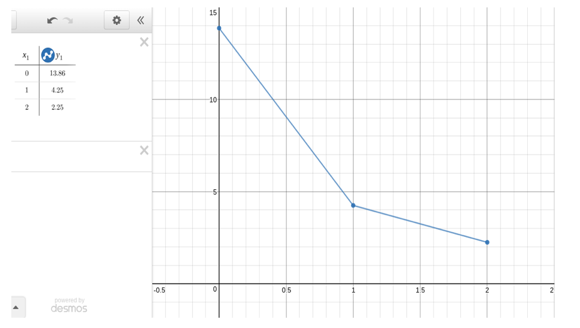
\includegraphics[width=14cm]{Student work sample 1.png}
    \subcaptionsetup{font=large}
    \subcaption*{This graph represents the rate of dissolution of the solute depending on the rate of stirring, with a controlled temperature of 17 degrees Celsius, with 0.2 Grams of copper sulfate, and 40 Milliliters of water for the solvent. 0 on the graph represents no stirring, 1 represents one rotation per second, and 2 represents two rotations per second.}
    \label{Table 2}
\end{figure*}
\begin{figure*}[h!]
    \centering
    \captionsetup{font=large}
    \caption*{\textit{Student Work Sample 2 (Group Using Google Charts)}}
    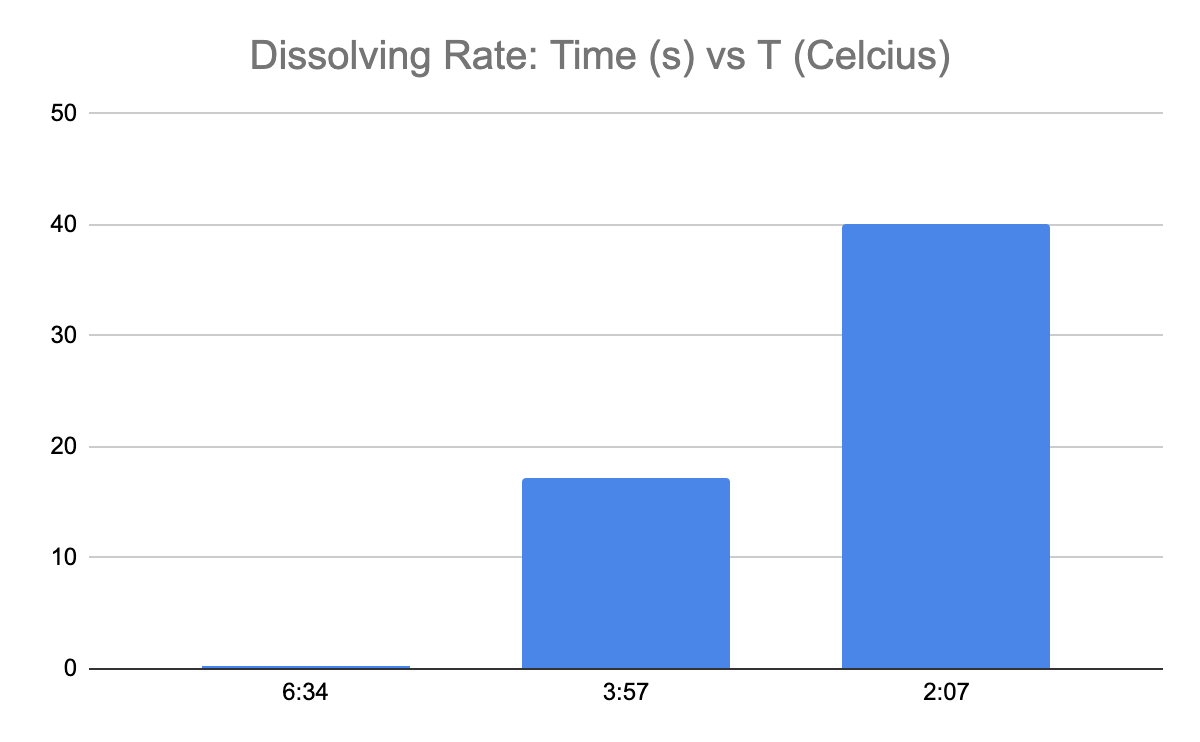
\includegraphics[width=13cm]{Student work sample 2.png}
    \label{Table 2.1}
\end{figure*}
\clearpage

\subsubsection*{Reducing Choices for Analyzing Data}
As discussed prior, providing templates for organization of thinking is a way to reduce or shorten the practice, time, or abstract qualities of an inquiry. Students can focus on key objectives in this way; the quality of learning. Yet, in addition to using templates, there are other ways to reduce or shorten data analysis and interpretation opportunities and still provide meaningful ways to practice this skill. Ms. G recognizes the key learning outcomes of developing skills for data interpretation result from students choosing and justifying their own methods. Due to this, she does not want to require a certain process; however, she also knows that opening data analysis to any method available could be overwhelming for some of her students. Prior to data analysis Ms. G determined several methods students could use. She knew that two of her three groups of students with the shortened/reduced assignments accommodation were in an Advanced Algebra class and that students in the other group were in a Pre-algebra math class. Knowing this she provided each group two methods that they could use to reason with their data. Each method would allow students to practice thinking mathematically in a way that made sense to them and would be aligned with their current skills, but that would also stretch and apply their prior knowledge. After some trial and error, which Ms. G encouraged as a way to decide, one of the groups chose to analyze their data using Desmos, a tool they had been exploring in their math class, and the other groups chose to use Google Charts to graph their variable(s) in relation to time. Samples of student work from these groups are in Table 2. Ms. G provides written directions for using Desmos, Excel and Google Charts to graph for all students in her class. Students also have the option of graphing by hand. Students are encouraged to ask questions of their peers and collaborate and share their knowledge of graphing and different programs, which they do readily. Additionally, for her groups that were assigned one or two variables, rather than three, the data they need to analyze and display is reduced. Ms. G uses frequent check-ins to monitor progress and emphasizes with the class the importance of developing and practicing this skill while using the tools, rather than perfection of the product.

\subsection*{\textit{\textbf{Data Interpretation and Modeling}}}
\textit{In this investigation Ms. G asks students to interpret data by creating a model of their results that shows why the variable(s) impacted dissolution in the way that the students determined experimentally. She communicates to all students that their models should represent what is happening at the molecular level, especially in relation to their variables, and incorporate the concept of energy, which has been a continuous topic of study in the class. Students create models in their groups and have choices about how to represent their understanding. Students can draw, or create a digital or physical model. Students with reduced and shortened assignments accommodations are engaged in a discussion at the beginning of this phase of the investigation to help them choose a model type that could represent their understanding, however, they are also provided the freedom to engage in trial and error. Ms. G provides these students a list of features that should be present in their model such as representations of different types and “levels” of energy, examples of how to represent a “particle” of a solution and or solute, etc. The three groups of students use the list to create their models.}

\subsubsection*{Developing Models to Increase and Demonstrate Understanding}
Developing and using models (NGSS SEP 2) is important for science learning and allows students to represent concepts to help them make sense, develop a deeper understanding, and communicate and refine their understanding, especially of abstract ideas (Park, Rodriquez, \& Campbell, 2019). Scientific modeling is dynamic and diverse. Examples include mathematical modeling, such as students creating an equation for photosynthesis after experimentation, and visual or physical representations, such as what Ms. G was requiring of her students; \textit{create a model that represents the dissolving process at a molecular level using the results of investigation and experimentation.} Her students had determined \textit{how} their variable(s) impacted dissolution, now they had to model the \textit{why}. Because Ms. G had already reduced the number of variables in the investigation to focus on purposeful practice, creating a model was also impacted. Her three groups of students would need to consider fewer variables in creating their model, allowing students more time to focus on representing and explaining the impacts of one or two variables, rather than three. However, Ms. G went beyond this in supporting students in this task. Ms. G created a list of key features of a completed model and provided this to her three groups. She did not tell students what to create or how, but assisted them in understanding factors that need to be represented. For instance, prior to creating their model they knew different ways that they could represent what was happening at a particulate level. Ms. G used their text, personal science notebooks, and class notes to remind them of other times they had drawn or used particulate level models. She also chose a particular model in their text that showed vibrating or energized atoms and asked students how the illustrator showed that the atoms were moving and what inputs (shown in the drawing) impacted this movement. These explicit questions tied to students’ prior academic knowledge and provided the groups an example and a starting point. Students could reference these illustrations as they made sense of and modeled their experimental findings in relation to what they were learning about the dissolution process. Additionally, they could use the checklist to determine their next steps in developing their model. 

\begin{figure} [h]
    \centering
    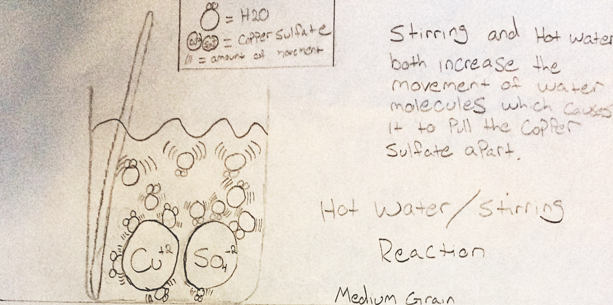
\includegraphics[width=\linewidth]{figure3.PNG}
    \captionsetup{font=large, labelfont=it}
    \caption*{\textit {Figure 3. Example of an Initial Molecular Level Model from a Group Examining Two Variables (Stirring and Temperature)}}
    \label{fig3}
\end{figure}

\begin{table*}[]
\captionsetup{font=large}
\caption*{\textbf{Table 3 \textit{Ms. G’s Rubric for the Content and Science Practice Objectives}}}
\label{tab:table-3}
\resizebox{\textwidth}{!}{%
\begin{tabular}{|llll|}
\hline
\multicolumn{4}{|l|}{\textbf{Molecular Level Dissolution Model Rubric}} \\
\multicolumn{4}{|l|}{\begin{tabular}[c]{@{}l@{}}Learning Objective: I can model the dissolution process as it happens \\ over time at a molecular level using scientific vocabulary.\end{tabular}} \\ \hline
\multicolumn{1}{|l|}{Model Factor} &
  \multicolumn{1}{l|}{Meeting} &
  \multicolumn{1}{l|}{Approaching} &
  Beginning \\ \hline
\multicolumn{1}{|l|}{1. Molecular Level} &
  \multicolumn{1}{l|}{\begin{tabular}[c]{@{}l@{}}Individual molecules \\ of both the solute and \\ solvent are indicated \\ and labeled.\end{tabular}} &
  \multicolumn{1}{l|}{\begin{tabular}[c]{@{}l@{}}Individual molecules \\ of both the solute and \\ solvent are indicated.\end{tabular}} &
  \begin{tabular}[c]{@{}l@{}}Particles in \\ a solution \\ are indicated.\end{tabular} \\ \hline
\multicolumn{1}{|l|}{2. Dissolving Process} &
  \multicolumn{1}{l|}{\begin{tabular}[c]{@{}l@{}}Model represents \\ solvent molecules \\ attaching to the solute \\ molecule and pulling \\ apart the solute \\ molecule by molecule.\end{tabular}} &
  \multicolumn{1}{l|}{\begin{tabular}[c]{@{}l@{}}Model represents \\ solvent molecules \\ attaching to the \\ solute molecule \\ and the solute \\ breaking apart.\end{tabular}} &
  \begin{tabular}[c]{@{}l@{}}Model represents \\ solvent molecules \\ attaching to the \\ solute molecule.\end{tabular} \\ \hline
\multicolumn{1}{|l|}{3. Time} &
  \multicolumn{1}{l|}{\begin{tabular}[c]{@{}l@{}}Model shows that \\ over time the solute \\ is pulled apart and is \\ dispersed throughout \\ the solvent.\end{tabular}} &
  \multicolumn{1}{l|}{\begin{tabular}[c]{@{}l@{}}Model shows that \\ over time the solute \\ breaks apart.\end{tabular}} &
  \begin{tabular}[c]{@{}l@{}}Model shows that \\ over time the solute \\ breaks apart.\end{tabular} \\ \hline
\multicolumn{1}{|l|}{\begin{tabular}[c]{@{}l@{}}4. Amount of \\ solvent vs. solute\end{tabular}} &
  \multicolumn{1}{l|}{\begin{tabular}[c]{@{}l@{}}A much larger \\ amount of solvent \\ molecules, compared \\ to the solute, are \\ represented in the model.\end{tabular}} &
  \multicolumn{1}{l|}{\begin{tabular}[c]{@{}l@{}}Solvent molecules \\ are equal to the solute \\ molecules represented \\ in the model.\end{tabular}} &
  \begin{tabular}[c]{@{}l@{}}A larger amount \\ of solute molecules \\ compared to \\ the solvent are \\ represented in \\ the model.\end{tabular} \\ \hline
\multicolumn{1}{|l|}{\begin{tabular}[c]{@{}l@{}}5. Electrostatic \\ Attraction\end{tabular}} &
  \multicolumn{1}{l|}{\begin{tabular}[c]{@{}l@{}}Model shows how \\ positive part of the \\ solvent surrounds \\ and attaches to \\ negative part of \\ the solute. Model \\ also represents the \\ opposite happening.\end{tabular}} &
  \multicolumn{1}{l|}{\begin{tabular}[c]{@{}l@{}}Model shows that \\ electrical charges are \\ involved in dissolution.\end{tabular}} &
  \begin{tabular}[c]{@{}l@{}}Model shows that \\ neutral and/or \\ nonpolar particles \\ are involved in \\ dissolution (or no \\ charge is shown).\end{tabular} \\ \hline
\multicolumn{1}{|l|}{6. Energy in System} &
  \multicolumn{1}{l|}{\begin{tabular}[c]{@{}l@{}}Model indicates that \\ increased energy in \\ the system, (from heat \\ and/or agitation) results \\ in more molecular \\ movement, more collisions, \\ and faster dissolution.\end{tabular}} &
  \multicolumn{1}{l|}{\begin{tabular}[c]{@{}l@{}}Model indicates that \\ increased energy in \\ the system results\\ in more molecular \\ movement and a \\ faster dissolution.\end{tabular}} &
  \begin{tabular}[c]{@{}l@{}}Model shows the \\ system has energy, \\ and the molecules \\ are moving or vibrating.\end{tabular} \\ \hline
\multicolumn{1}{|l|}{\begin{tabular}[c]{@{}l@{}}7. Surface Area \\ (If applicable)\end{tabular}} &
  \multicolumn{1}{l|}{\begin{tabular}[c]{@{}l@{}}Model shows that higher \\ surface area to volume ratios \\ result in faster dissolution.\end{tabular}} &
  \multicolumn{1}{l|}{\begin{tabular}[c]{@{}l@{}}Model shows that \\ solute surface area \\ impacts dissolution rate.\end{tabular}} &
  \begin{tabular}[c]{@{}l@{}}Model shows that lower \\ surface area to volume \\ ratios result in faster \\ dissolution.\end{tabular} \\ \hline
\end{tabular}%
}
\end{table*}
\clearpage
\subsection*{\textit{\textbf{Evaluation of Learning and Practice}}}
\textit{Ms. G created a rubric (Table 3) that aligned with one of the science practices and her content learning objectives. Her rubric focused on} NGSS Science and Engineering Practice 2: Developing and Using Models, \textit{specifically, developing a model to explain experimental results related to the kinetics of dissolution. She shared the rubric with her students and asked them to use it prior to submitting the models to self-assess and potentially revise their work. After this, students submitted their models for her assessment. Ms. G used the rubric to evaluate and provide feedback to each group as well as to assign a grade (five points per model factor). Ms. G highlighted in yellow sections of the rubric related to the model that needed more detail or attention. Ms. G also collected student notebooks to offer feedback on how they planned and carried out an investigation (Practice 3) and analyzed and interpreted data (Practice 4). When Ms. G was finished with her evaluation and feedback, she returned the notebooks, models, and completed rubrics to students and provided them an opportunity for further revision based on her feedback. The six students with the shortened/reduced assignments accommodation were assessed in the same manner as her general education students. They also had the same opportunities to demonstrate mastery through revision and use of feedback. These groups used the highlighted areas of the rubric to further revise and develop their model before giving it back to Ms. G for another round of evaluation. All students participated in as many revision/feedback cycles as they needed to demonstrate mastery.}

\subsubsection*{Evaluation and Feedback When Reducing or Shortening Investigation Tasks}
Shortening and reducing assignments while maintaining quality of work is an accommodation for students with learning disabilities that is designed to allow access to the same learning objectives and opportunities as general education students, but reduces practice in a purposeful way. It can be difficult for teachers to evaluate students equitably who have this accommodation (Ketterlin-Geller, Alonzo, Braun-Monegan, \& Tindal, 2007). Evaluation of student learning should be related to demonstration of understanding and mastery of the learning objectives. If students have access, through accommodation, they should be evaluated on the objectives using the same criteria as general education students. A key question Ms. G asked was, did her six students with learning disabilities meet the learning objectives? In this case, did they provide evidence that they understood dissolution at a particulate level? Did they provide evidence that they practiced and engaged in the NGSS SEPs? Ms. G evaluated student developed models with the same rubric as her general education students to determine if they met the content objective. To promote deeper understanding she required that all students demonstrate mastery of this objective by providing feedback and time for revision based on the rubric. She additionally provided students feedback on the objectives related to the NGSS SEPs 3 and 4 through reading their notebooks but did not assign a grade related to this portion of her objectives. Ms. G emphasized to all of her students that they were to continue practicing their science process skills, taking her feedback into account, to become more adept at using an investigative and experimental approach to gather and interpret evidence, and to create and evaluate scientific explanations, including models. 

\section*{Conclusion}
In Ms. G’s class students who received the shortened/reduced assignments accommodation were afforded accessible opportunities to practice and improve their science process skills and dispositions while developing grade-level content understanding during an inquiry investigation. A summary of the strategies Ms. G used to support her students is illustrated in Figure 4 and detailed in Table 4. In Ms. G’s class, all students practiced planning and carrying out an investigation, analyzing and interpreting data, and developing and using models during an inquiry investigation while learning about the process of dissolution on a particulate level. 

\begin{figure} [h]
    \centering
    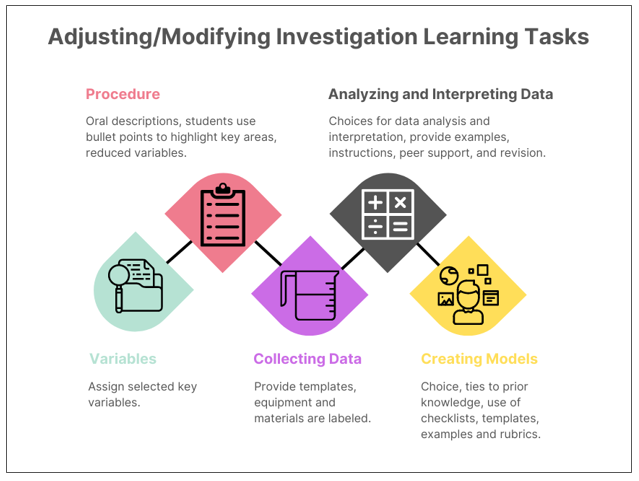
\includegraphics[width=13cm]{figure4.PNG}
    \captionsetup{font=large}
    \caption*{\textit{\textbf{Figure 4. Flowchart of Investigation Steps and Strategies}}}
    \label{fig:fig4}
\end{figure}

\clearpage

% Please add the following required packages to your document preamble:
% \usepackage{graphicx}
\begin{table*}[t]
\captionsetup{font=large}
\caption*{\textbf{Table 4:\textit{ Strategies for Adjusting/Modifying Investigation Learning Tasks}}}
\label{tab:table-4}
\resizebox{\textwidth}{!}{%
\begin{tabular}{|l|l|l|}
\hline
\multicolumn{1}{|c|}{\textbf{Learning Tasks}} &
  \multicolumn{1}{c|}{\textbf{Description of Task}} &
  \multicolumn{1}{c|}{\textbf{Strategy}} \\ \hline
\begin{tabular}[c]{@{}l@{}}Investigation Variables \\ (NGSS Science Practice 3)\end{tabular} &
  \begin{tabular}[c]{@{}l@{}}Students investigate variables \\ related to a phenomenon.\end{tabular} &
  \begin{tabular}[c]{@{}l@{}}Assign selected key variables. \\ Determine the abstraction of \\ each variable and assign \\ variables related to this.\end{tabular} \\ \hline
\begin{tabular}[c]{@{}l@{}}Investigation Procedure \\ (NGSS Science Practice 3)\end{tabular} &
  \begin{tabular}[c]{@{}l@{}}Students design a procedure \\ for an investigation.\end{tabular} &
  \begin{tabular}[c]{@{}l@{}}Students describe their \\ procedure orally and use bullet \\ points to highlight key areas \\ of procedure. Students design \\ procedure for selected variables.\end{tabular} \\ \hline
\begin{tabular}[c]{@{}l@{}}Collecting Data \\ (NGSS Science Practice 3)\end{tabular} &
  \begin{tabular}[c]{@{}l@{}}Students create data tables \\ appropriate to their procedure. \\ Students collect experimental \\ data.\end{tabular} &
  \begin{tabular}[c]{@{}l@{}}Provide varied templates for \\ data tables, allow student choice. \\ Students use or modify an existing \\ template. Materials and equipment \\ are labeled, visuals and written \\ instructions are provided as needed.\end{tabular} \\ \hline
\begin{tabular}[c]{@{}l@{}}Analyzing and Interpreting \\ Data (NGSS Science \\ Practice 3, 4, 5)\end{tabular} &
  \begin{tabular}[c]{@{}l@{}}Students organize, calculate, \\ and display their data. Students \\ find patterns in their data and \\ determine evidence (key data).\end{tabular} &
  \begin{tabular}[c]{@{}l@{}}Provide two or three choices for \\ data analysis and interpretation \\ aligned with mathematical prior \\ knowledge. Provide examples of \\ each type of data analysis. Use a \\ gallery walk prior to data \\ interpretation; students see how \\ other students analyzed data. \\ Encourage revision.\end{tabular} \\ \hline
\begin{tabular}[c]{@{}l@{}}Creating Models \\ (NGSS Science Practice 2)\end{tabular} &
  \begin{tabular}[c]{@{}l@{}}Students develop a model to \\ explain experimental results.\end{tabular} &
  \begin{tabular}[c]{@{}l@{}}Students are given a choice of \\ how create model. Students are \\ provided a template, checklist, \\ examples and/or rubric. Use of \\ explicit questions and examples \\ to tie prior knowledge and \\ academic experiences to what \\ the model should represent.\end{tabular} \\ \hline
\end{tabular}%
}
\end{table*}

\include{} 
\section*{References}\par 

\leftskip 0.25in
\parindent -0.25in 
%%%

Bransford, J., \& Donovan, S. (2005). \textit{How Students Learn: Science in the Classroom}. National Research Council. Washington, DC: The National Academies Press.\\

Chittleborough, G., \& Treagust, D. (2009) Why Models are Advantageous to Learning Science.
\textit{Educación Química, (20)}1, 12-17.\\

Gutierrez, Y. (2013). \textit{Co-teachers and parents’ perceptions of shortened assignments for \\learning disabled students}. (Doctoral dissertation) Retrieved from: \url{https://www.proquest.com/openview/fb285af7d0270bbd2b87f58bfaab7954/1?pq-origsite=gscholar\&cbl=18750}\\

Instructional Leadership for Science Practices. (n.d.) Definitions of NGSS Science Practices. \url{https://www.sciencepracticesleadership.com/}\\

Ketterlin-Geller, L. R., Alonzo, J., Braun-Monegan, J., \& Tindal, G. (2007). Recommendations for accommodations: Implications of \\(in)consistency. \textit{Remedial and Special Education, 28}(4), 194–206.\\

Martin-Hansen, L. (2002). Defining inquiry: Exploring the many types of inquiry in the science classroom. \textit{The Science Teacher, \\69}(2), 34-37. \\

McGrath, A.L., \& Hughes, M. T. (2018). Students with learning disabilities in inquiry-based science classrooms: A cross-case analysis. \textit{Learning Disability Quarterly 41}(3), 131–143.

Melber, L. (2004). Inquiry for everyone: Authentic science experiences for students with special needs. \textit{Teaching Exceptional Children Plus, 1}(2), Article 4.\\

National Research Council. (1996). \textit{National science education standards}. Washington, DC: National Academy Press.\\

NGSS Lead States. (2013). Next Generation Science Standards: For States, By States. Washington, DC: The National Academies Press.\\

O’Rourke, J., \& Houghton, S. (2009). The perceptions of secondary teachers and students about the implementation of an inclusive classroom model for students with mild disabilities.
\textit{Australian Journal of Teacher Education, 31}(1), Article 3.\\

Park, B., Rodriquez, L., \& Campbell, T. (2019). Using models to teach science. \textit{The Science Teacher. 87}(4), Article 2.\\

Rizzo, K. L., \& Taylor, J. C. (2016). Effects of inquiry-based instruction on science achievement for students with disabilities: an analysis of the literature. \textit{Journal of Science Education for Students with Disabilities, 19}(1), Article 2.\\

Sampson, V., Carafano, P., Enderle, P., Fannin, S., Grooms, J., Southerland, S., Stallworth, C., \& Williams, K. (2015). \textit{Argument-Driven Inquiry in Chemistry: Lab Investigations for Grades 9-12}. Arlington, Virginia: NSTA Press, National Science Teachers Association\\

Therrien, W. J., Taylor, J. C., Hosp, J. L., Kaldenberg, E. R., \& Gorsh, J. (2011). Science instruction for students with learning disabilities: A meta-analysis. \textit{Learning Disabilities Research \& Practice, 26}, 188–203.

\end{large}
\end{document}
